\documentclass[a4paper]{article}

\usepackage[UTF8]{ctex}
\usepackage[a4paper,margin=1in]{geometry}
\usepackage{graphicx}
\usepackage{float}
\usepackage{listings}
\usepackage{longtable}
\usepackage{booktabs}
\usepackage{hyperref}
\usepackage{fancyhdr}
\usepackage{lastpage}
\usepackage{color}
\usepackage{indentfirst}        % 首段缩进
\setlength{\parindent}{2em}     % 缩进2字符
\usepackage{zhnumber}           % 中文编号
\usepackage[dvipsnames]{xcolor}

%\newcommand{\college}{中山大学计算机学院}
\newcommand{\projname}{数据库系统原理实验|实验八}
\newcommand{\reporttitle}{数据库应用开发实验}
\newcommand{\stuno}{23336179}
\newcommand{\authorname}{马福泉}
\newcommand{\major}{计算机科学与技术}
\newcommand{\adviser}{赖韩江}
\newcommand{\startdate}{2025年11月13日}
\newcommand{\labenddate}{2025年11月17日}
\newcommand{\labroom}{B202}

\pagestyle{fancy} % 使用 fancyhdr 风格
\fancyhf{}      % 清空默认的页眉页脚

% 设置页眉
\fancyhead[L]{\kaishu \projname}      % 左侧页眉显示项目名称
\fancyhead[C]{\kaishu \reporttitle}    % 中间页眉显示报告标题
\fancyhead[R]{\kaishu \authorname} % 右侧页眉显示作者姓名

% 设置页脚
\fancyfoot[C]{第 \thepage 页，共 \pageref{LastPage} 页} % 中间页脚显示页码

% 去除页眉页脚与正文之间的分隔线
\renewcommand{\headrulewidth}{0.4pt}
\renewcommand{\footrulewidth}{0pt}

% 设置文档背景颜色
\definecolor{mybgcolor}{RGB}{0, 0, 0} % 定义背景颜色
\definecolor{NavyBlue}{RGB}{0,0,128} % 添加颜色定义
% \pagecolor{mybgcolor} % 设置背景颜色

% listing 配置rust
% \lstdefinelanguage{Rust}{
%   keywords={fn, let, mut, struct, enum, impl, pub, use, mod, trait, where},
%   keywordstyle=\color{NavyBlue},
%   comment=[l]{//},
%   commentstyle=\color{gray},
% }
% \lstset{language=Rust}

\lstset{
  basicstyle=\ttfamily\small,
  keywordstyle=\color{NavyBlue},
  commentstyle=\color{gray},
  stringstyle=\color{red},
  showstringspaces=false,
  extendedchars=false, % 关键：不处理中文
  breaklines=true,
  language=Python
}

\begin{document}

% 封面
\begin{titlepage}
    \centering
    
\includegraphics[width=10cm]{img/SYSULogo.png}

    \vspace{1em}
    %{\Large \college \par}
    \vspace{1em}
    {\Large \kaishu \projname \par}
    \vspace{3em}

    

    
    {\fontsize{40pt}{42pt}\kaishu \selectfont \boldmath \reporttitle\par}
    \vspace*{\fill}

    \begin{center}
    {\Large
    \makebox[5em][s]{学号}:\underline{\makebox[15em][c]{\kaishu \stuno}}\\[1em]
    \makebox[5em][s]{姓名}:\underline{\makebox[15em][c]{\kaishu \authorname}}\\[1em]
    \makebox[5em][s]{专业}:\underline{\makebox[15em][c]{\kaishu \major}}\\[1em]
    \makebox[5em][s]{课程教师}:\underline{\makebox[15em][c]{\kaishu \adviser}}\\[1em]
    \makebox[5em][s]{起始日期}:\underline{\makebox[15em][c]{\kaishu \startdate}}\\[1em]
    \makebox[5em][s]{结束日期}:\underline{\makebox[15em][c]{\kaishu \labenddate}}\\[1em]
    \makebox[5em][s]{实验地点}:\underline{\makebox[15em][c]{\kaishu \labroom}}
    }
    \end{center}

    \vspace*{\fill}
\end{titlepage}

% 目录
\tableofcontents
\newpage

\section{实验概述}

\subsection{实验目的}
掌握使用程序设计语言访问数据库。

\subsection{实验内容}
使用pymssql连接图书借阅数据库系统JY，并利用pymssql执行下述操作：
\begin{enumerate}
    \item 在reader表增加一条数据：'r0020', '王小明', '男', '临床医学系'；
    \item 将reader表新增数据'r0020'的部门更新为'护理系'；
    \item 查询价格高于50的书籍，并打印；
    \item 查询信息工程系的读者，并打印；
    \item 删除reader表新增数据'r0020'；
    \item 打印图书表book、读者表reader的所有数据。
\end{enumerate}

\section{实验报告}

\subsection{环境准备}

\subsubsection{Python环境配置}
首先在Windows命令提示符或PowerShell中安装pymssql库：
\begin{lstlisting}
pip install pymssql
\end{lstlisting}

\subsubsection{SQL Server端口配置}

在进行数据库连接之前，需要确保SQL Server的TCP/IP协议已启用并正确配置端口。

\textbf{步骤1：打开SQL Server配置管理器}

\textbf{步骤2：检查TCP/IP端口配置}
\begin{enumerate}
    \item 展开"SQL Server网络配置" → "MSSQLSERVER的协议"
    \item 右键点击"TCP/IP" → 属性 → IP地址选项卡
    \item 滚动到最底部，查看"IPAll"部分的"TCP端口"
    \item 确认端口是否为1433（SQL Server默认端口）
\end{enumerate}

\begin{figure}[H]
    \centering
    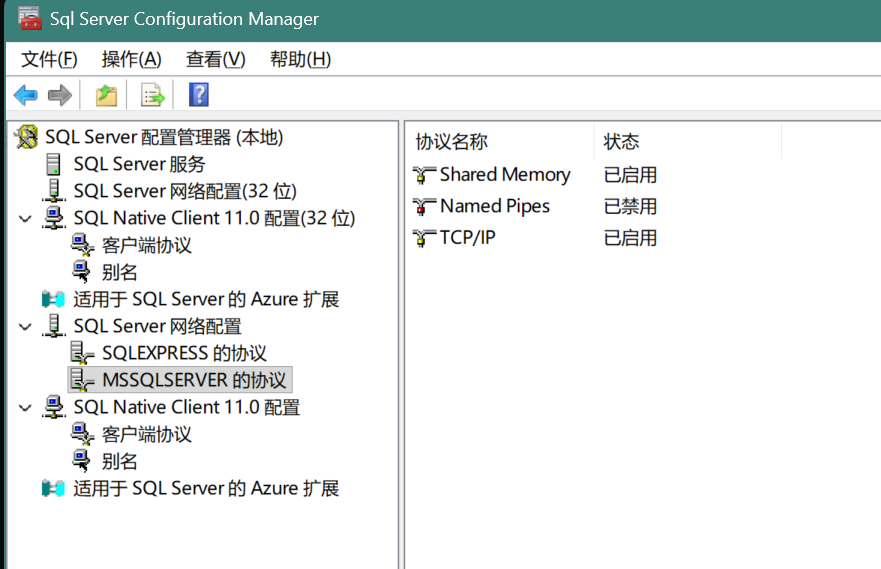
\includegraphics[width=0.8\textwidth]{img/set1433.png}
    \caption{设置TCP/IP端口为1433的配置截图}
\end{figure}

\textbf{步骤3：启用TCP/IP协议}

如果TCP/IP协议未启用，需要进行以下操作：
\begin{enumerate}
    \item 在SQL Server配置管理器中
    \item 右键点击"TCP/IP" → 选择"启用"
    \item 配置TCP/IP协议：
    \begin{itemize}
        \item 右键点击"TCP/IP" → 属性 → IP地址选项卡
        \item 确保所有IP地址的"活动"和"已启用"都设置为"是"
        \item 在"IPAll"部分设置"TCP端口"为1433
    \end{itemize}
\end{enumerate}

\textbf{步骤4：重启SQL Server服务}

配置完成后需要重启SQL Server服务：
\begin{enumerate}
    \item 在SQL Server配置管理器中，选择"SQL Server服务"
    \item 右键点击"SQL Server (MSSQLSERVER)" → 重新启动
\end{enumerate}

\begin{figure}[H]
    \centering
    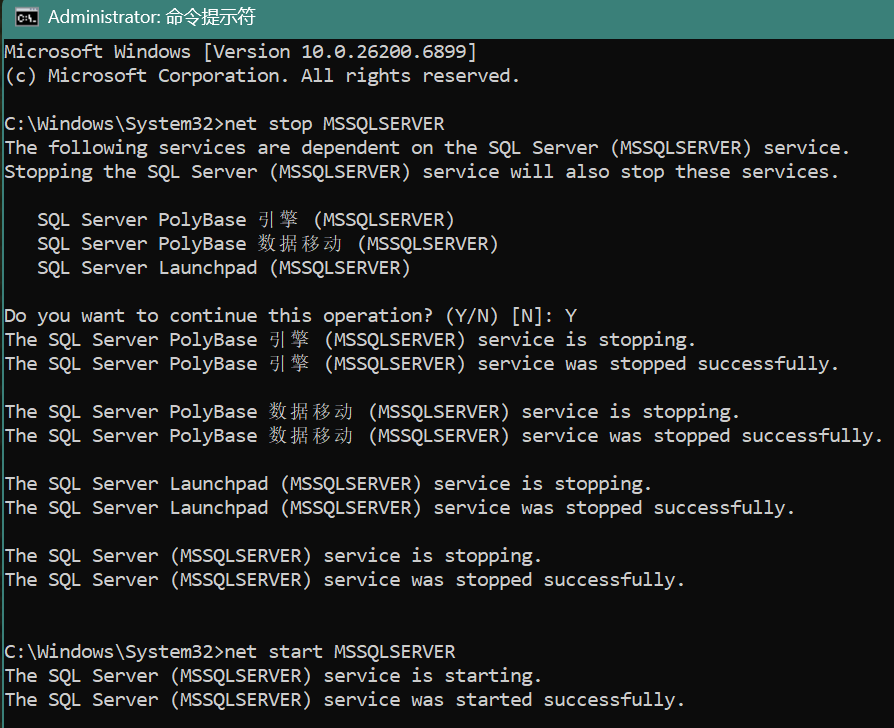
\includegraphics[width=0.8\textwidth]{img/reboot.png}
    \caption{重启SQL Server服务截图}
\end{figure}

\textbf{步骤5：验证端口配置}

如果端口不是1433，在Python连接代码中需要指定端口号：

\begin{lstlisting}
# 在连接字符串中指定端口
conn = pymssql.connect(
    server='FORTUNE,1433',  # 服务器名称,端口号
    database='JY'
)
\end{lstlisting}

\begin{figure}[H]
    \centering
    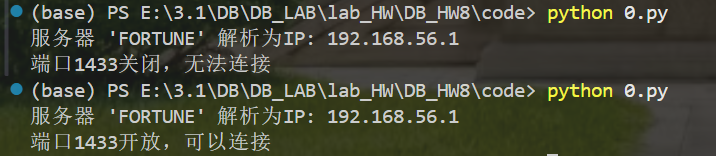
\includegraphics[width=0.8\textwidth]{img/success.png}
    \caption{成功连接1433端口的截图}
\end{figure}

\subsection{步骤0：数据库连接配置}

在完成SQL Server端口配置后，建立与图书借阅数据库系统JY的连接。

首先创建测试连接的代码文件\texttt{0.py}：

\begin{lstlisting}
import pymssql

def test_connection():
    try:
        conn = pymssql.connect(server='FORTUNE', database='JY')
        cursor = conn.cursor()
        cursor.execute("SELECT @@VERSION")
        version = cursor.fetchone()
        print(f"连接成功! SQL Server版本: {version[0]}")
        conn.close()
        return True
    except Exception as e:
        print(f"连接失败: {e}")
        return False

if __name__ == "__main__":
    test_connection()
\end{lstlisting}

\textbf{执行步骤：}
\begin{enumerate}
    \item 在命令提示符中进入代码目录
    \item 运行：\texttt{python 0.py}
    \item 确认连接成功
\end{enumerate}

\textbf{执行结果：}

\begin{figure}[H]
    \centering
    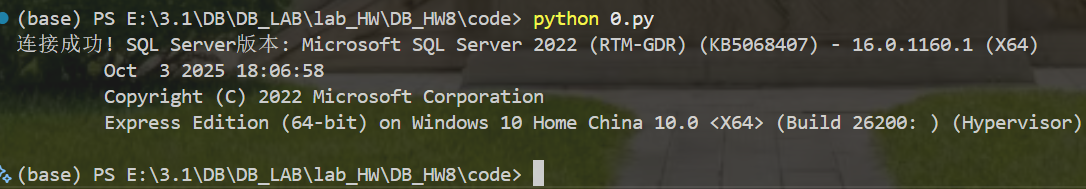
\includegraphics[width=0.8\textwidth]{img/0.png}
    \caption{数据库连接成功截图}
\end{figure}

\subsection{步骤1：在reader表增加一条数据}

创建文件\texttt{1.py}，在reader表中插入新记录'r0020', '王小明', '男', '临床医学系'：

\begin{lstlisting}
# 在reader表增加一条数据
import pymssql

def add_reader():
    """添加读者记录"""
    try:
        # 连接数据库
        conn = pymssql.connect(server='FORTUNE', database='JY', port=1433)
        cursor = conn.cursor()
        print("数据库连接成功!")
        
        sql = "INSERT INTO reader (reader_id, reader_name, reader_sex, reader_department) VALUES (%s, %s, %s, %s)"
        values = ('r0020', '王小明', '男', '临床医学系')
        cursor.execute(sql, values)
        conn.commit()
        
        print("任务1：成功添加读者记录")
        print(f"添加的数据: reader_id='r0020', reader_name='王小明', reader_sex='男', reader_department='临床医学系'")
        
        # 验证插入结果
        cursor.execute("SELECT * FROM reader WHERE reader_id = 'r0020'")
        result = cursor.fetchone()
        print(f"验证结果: {result}")
        
        conn.close()
        return True
        
    except Exception as e:
        print(f"任务1执行失败: {e}")
        return False

if __name__ == "__main__":
    add_reader()
\end{lstlisting}

\textbf{执行结果：}

\begin{figure}[H]
    \centering
    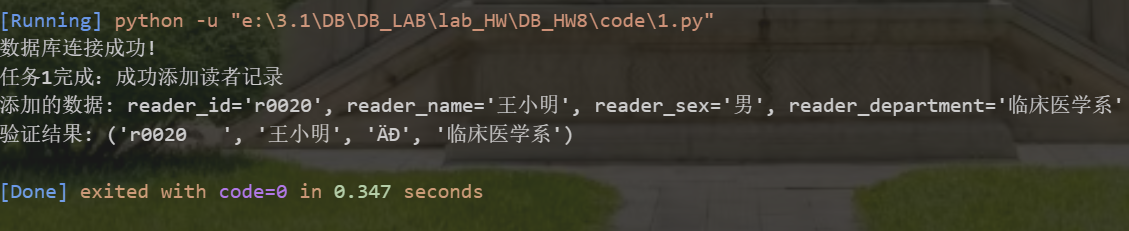
\includegraphics[width=0.8\textwidth]{img/1.png}
    \caption{插入读者数据结果截图}
\end{figure}

\subsection{步骤2：更新reader表数据}

创建文件\texttt{2.py}，将reader表新增数据'r0020'的部门更新为'护理系'：

\begin{lstlisting}
# 任务2：更新读者部门信息
import pymssql

def update_reader_department():
    """更新读者部门信息"""
    try:
        # 连接数据库
        conn = pymssql.connect(server='FORTUNE', database='JY', port=1433)
        cursor = conn.cursor()
        print("数据库连接成功!")
        
        sql = "UPDATE reader SET reader_department = %s WHERE reader_id = %s"
        values = ('护理系', 'r0020')
        cursor.execute(sql, values)
        conn.commit()
        
        print("任务2：成功更新读者部门")
        print(f"将读者'r0020'的部门从'临床医学系'更新为'护理系'")
        
        # 验证更新结果
        cursor.execute("SELECT * FROM reader WHERE reader_id = 'r0020'")
        result = cursor.fetchone()
        print(f"更新后的读者信息: {result}")
        
        conn.close()
        return True
        
    except Exception as e:
        print(f"任务2执行失败: {e}")
        return False

if __name__ == "__main__":
    update_reader_department()
\end{lstlisting}

\textbf{执行结果：}

\begin{figure}[H]
    \centering
    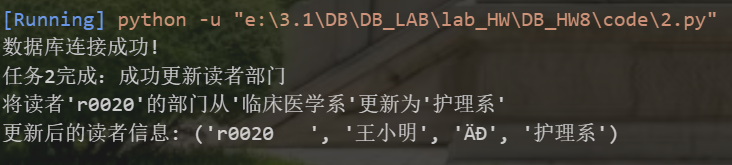
\includegraphics[width=0.8\textwidth]{img/2.png}
    \caption{更新读者部门结果截图}
\end{figure}

\subsection{步骤3：查询价格高于50的书籍}

创建文件\texttt{3.py}，查询价格高于50的书籍，并打印：

\begin{lstlisting}
#任务3：查询价格高于50的书籍
import pymssql

def query_expensive_books():
    """查询价格高于50的书籍"""
    try:
        # 连接数据库
        conn = pymssql.connect(server='FORTUNE', database='JY', port=1433)
        cursor = conn.cursor()
        print("数据库连接成功!")
        
        # 查询价格高于50的书籍
        sql = "SELECT * FROM book WHERE book_price > 50"
        cursor.execute(sql)
        books = cursor.fetchall()
        
        print("任务3结果：价格高于50的书籍")
        print("=" * 60)
        
        if books:
            for book in books:
                print(f"图书ID: {book[0]}, 书名: {book[1]}, 价格: {book[2]}")
            print(f"共找到 {len(books)} 本价格高于50的书籍")
        else:
            print("没有找到价格高于50的书籍")
            
        print("=" * 60)
        
        conn.close()
        return True
        
    except Exception as e:
        print(f"任务3执行失败: {e}")
        return False

if __name__ == "__main__":
    query_expensive_books()
\end{lstlisting}

\textbf{执行结果：}

\begin{figure}[H]
    \centering
    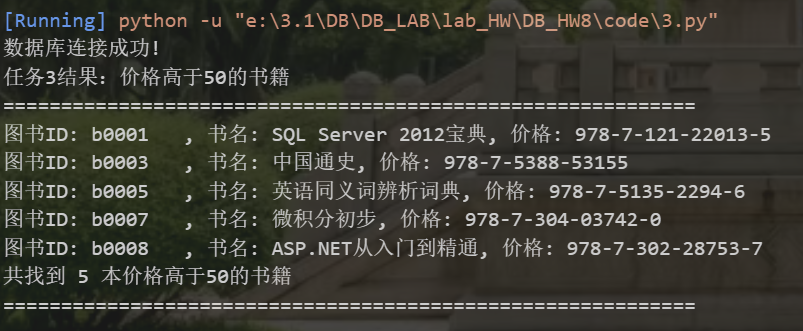
\includegraphics[width=0.8\textwidth]{img/3.png}
    \caption{查询价格高于50的书籍结果截图}
\end{figure}

\subsection{步骤4：查询信息工程系的读者}

创建文件\texttt{4.py}，查询信息工程系的读者，并打印：

\begin{lstlisting}
# 任务4：查询信息工程系的读者
import pymssql

def query_info_engineering_readers():
    """查询信息工程系的读者"""
    try:
        # 连接数据库
        conn = pymssql.connect(server='FORTUNE', database='JY', port=1433)
        cursor = conn.cursor()
        print("数据库连接成功!")
        
        # 查询信息工程系的读者 - 使用正确的列名
        sql = "SELECT * FROM reader WHERE reader_department = '信息工程系'"
        cursor.execute(sql)
        readers = cursor.fetchall()
        
        print("任务4结果：信息工程系的读者")
        print("=" * 60)
        
        if readers:
            for reader in readers:
                print(f"读者ID: {reader[0]}, 姓名: {reader[1]}, 性别: {reader[2]}, 部门: {reader[3]}")
            print(f"共找到 {len(readers)} 位信息工程系的读者")
        else:
            print("没有找到信息工程系的读者")
            
        print("=" * 60)
        
        conn.close()
        return True
        
    except Exception as e:
        print(f"任务4执行失败: {e}")
        return False

if __name__ == "__main__":
    query_info_engineering_readers()
\end{lstlisting}

\textbf{执行结果：}

\begin{figure}[H]
    \centering
    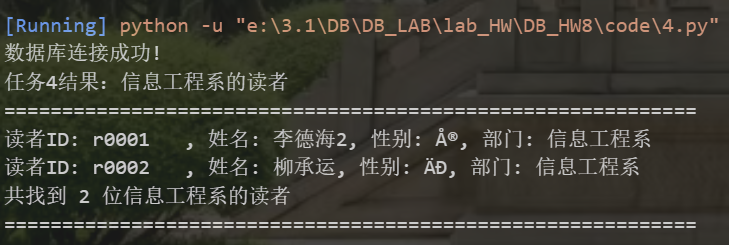
\includegraphics[width=0.8\textwidth]{img/4.png}
    \caption{查询信息工程系读者结果截图}
\end{figure}

\subsection{步骤5：删除reader表新增数据}

创建文件\texttt{5.py}，删除reader表新增数据'r0020'：

\begin{lstlisting}
# 任务5：删除读者记录
import pymssql

def delete_reader():
    """删除读者记录"""
    try:
        # 连接数据库
        conn = pymssql.connect(server='FORTUNE', database='JY', port=1433)
        cursor = conn.cursor()
        print("数据库连接成功!")
        
        # 先确认要删除的记录存在
        cursor.execute("SELECT * FROM reader WHERE reader_id = 'r0020'")
        reader = cursor.fetchone()
        
        if reader:
            print(f"找到要删除的读者记录: {reader}")
            
            # 删除读者记录
            sql = "DELETE FROM reader WHERE reader_id = %s"
            cursor.execute(sql, ('r0020',))
            conn.commit()
            
            print("任务5完成：成功删除读者记录")
            print(f"已删除读者ID为'r0020'的记录")
            
            # 验证删除结果
            cursor.execute("SELECT * FROM reader WHERE reader_id = 'r0020'")
            result = cursor.fetchone()
            if not result:
                print("确认读者记录已成功删除")
            else:
                print("警告：读者记录可能未成功删除")
        else:
            print("未找到读者记录r0020，无需删除")
        
        conn.close()
        return True
        
    except Exception as e:
        print(f"任务5执行失败: {e}")
        return False

if __name__ == "__main__":
    delete_reader()
\end{lstlisting}

\textbf{执行结果：}

\begin{figure}[H]
    \centering
    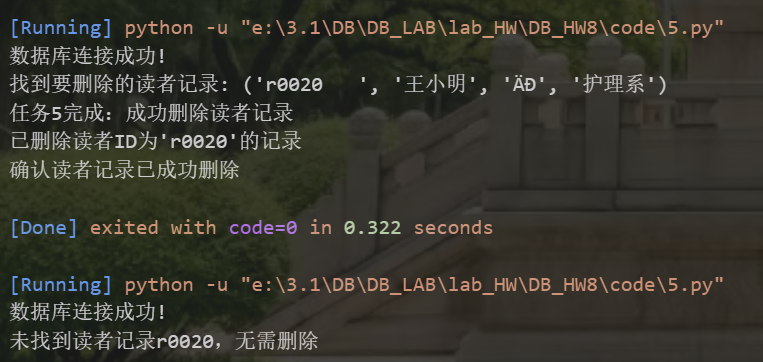
\includegraphics[width=0.8\textwidth]{img/5.png}
    \caption{删除读者数据结果截图}
\end{figure}

\subsection{步骤6：打印所有数据}

创建文件\texttt{6.py}，打印图书表book、读者表reader的所有数据：

\begin{lstlisting}
#任务6：打印所有图书和读者数据
import pymssql

def print_all_data():
    """打印所有图书和读者数据"""
    try:
        # 连接数据库
        conn = pymssql.connect(server='FORTUNE', database='JY', port=1433)
        cursor = conn.cursor()
        print("数据库连接成功!")
        
        # 打印图书表数据
        print("任务6结果：图书表所有数据")
        print("=" * 60)
        cursor.execute("SELECT * FROM book")
        books = cursor.fetchall()
        
        if books:
            for book in books:
                print(f"图书ID: {book[0]}, 书名: {book[1]}, 价格: {book[2]}")
            print(f"图书表共有 {len(books)} 条记录")
        else:
            print("图书表中没有数据")
        
        # 打印读者表数据
        print("\n任务6结果：读者表所有数据")
        print("=" * 60)
        cursor.execute("SELECT * FROM reader")
        readers = cursor.fetchall()
        
        if readers:
            for reader in readers:
                print(f"读者ID: {reader[0]}, 姓名: {reader[1]}, 性别: {reader[2]}, 部门: {reader[3]}")
            print(f"读者表共有 {len(readers)} 条记录")
        else:
            print("读者表中没有数据")
            
        print("=" * 60)
        
        conn.close()
        return True
        
    except Exception as e:
        print(f"任务6执行失败: {e}")
        return False

if __name__ == "__main__":
    print_all_data()
\end{lstlisting}

\textbf{执行方式：}
在命令提示符中运行：\texttt{python 6.py}

\textbf{执行结果：}

\begin{figure}[H]
    \centering
    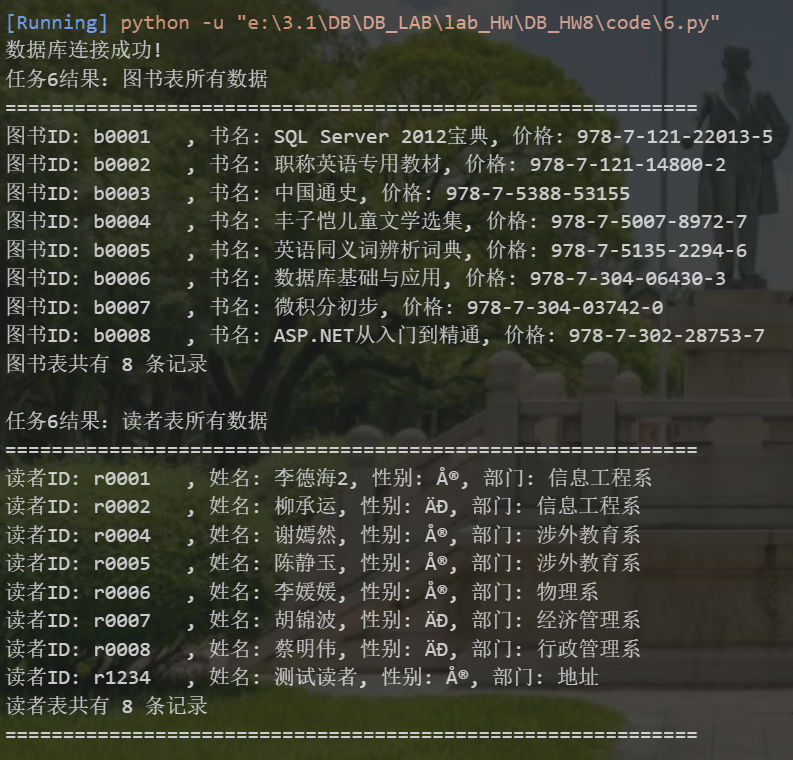
\includegraphics[width=0.8\textwidth]{img/6.png}
    \caption{打印所有数据结果截图}
\end{figure}

\subsection{实验总结}

\subsubsection{遇到的困难和解决}

\textbf{困难：}初期连接数据库时频繁出现连接失败的错误，无法建立与SQL Server的有效连接。

\textbf{解决方案：}
\begin{itemize}
    \item 检查并启用SQL Server的TCP/IP协议
    \item 确认端口1433的正确配置
    \item 重启SQL Server服务使配置生效
    \item 使用简洁的连接字符串：\texttt{pymssql.connect(server='FORTUNE', database='JY')}
\end{itemize}

\textbf{困难：}程序在出现异常时可能导致数据库连接未正确关闭，影响系统性能。

\textbf{解决方案：}
\begin{itemize}
    \item 使用try-except-finally结构确保连接和游标的正确关闭
    \item 在每个数据库操作函数中添加完善的异常处理
    \item 在插入、更新、删除操作后及时提交事务（\texttt{conn.commit()}）
\end{itemize}

\subsubsection{收获与反思}

通过本次实验，我获得了以下重要收获和体会：
\begin{itemize}
    \item 熟练掌握使用Python的pymssql库连接和操作SQL Server数据库
    \item 学会编写标准的CRUD（增删改查）操作代码
    \item 理解了参数化查询的重要性和使用方法
    \item 学会了将复杂的实验任务分解为独立的功能模块，便于调试和维护
    \item 在遇到连接问题时，通过查阅文档和逐步调试，最终找到了正确的解决方案
\end{itemize}

本次实验不仅提升了我的数据库编程技能，更重要的是培养了我解决实际问题的能力和系统性思维方式，为今后学习奠定了良好基础。

\end{document}